% !TEX root = MainDocument.tex
\thispagestyle{firstPage}

\section{Der Analog- Digital- Wandler}
\label{sec:ad-wandler}

Im ersten Teil der Arbeit geht es um die digitale Messung analoger Größen des Moduls.
Das Framework wurde am Beispiel der Temperaturmessung des neuen Moduls entwickelt, demnach soll dieser Anwendungsfall hier genauer beschrieben werden.

Das Messen analoger Größen ist einer der häufigsten Anwendungsfälle eingebetteter Systeme. 
Die meisten Größen unseres Umfeldes sind analoger Natur: Stimmen, Bilder, Druck und eben Temperatur.
Die Verarbeitung analoger Signale ist schwierig, kostspielig und störanfällig.
Deswegen werden Analog- Digital Wandler eingesetzt, um robuste und performante Anwendungen zu gewährleisten.

Zunächst sei hier gesagt, dass mithilfe eines \ac{adc} nicht nur die Temperatur gemessen werden kann.
Aufgabe des Bauteils ist es, eine analoge Spannung in einen digitalen Wert zu formen.
Dazu wird über eine über ein auf externe Reize reagierendes Bauteil abfallende Spannung an die Eingänge des Bauteils geschalten.
Diese Spannung kann aber auch von einem beliebigen Sensor stammen.
Abhängig davon, ob dieser Sensor oder externe Bauteil auf Temperatur oder eben andere Reize reagiert, kann der \ac{adc} verschiedene Größen messen.

Grob gesagt misst ein \ac{adc} die anliegenede Messspannung im Verhältnis zu einer anliegenden Referenzsspannung.
Das Bauteil bildet danach das Verhältnis von anliegender Messspannung zu Referenzsspannung.
Daraus wird ein einheitenloser Wert gebildet (siehe auch \autoref{eq:adc-messung}, die Einheit kürzt sich).

Das Verhältnis diesen Wertes zum maximal messbaren Wert des Bauteils entspricht dem Verhältnis der beiden vorhin genannten Spannungen (siehe \autoref{eq:adc-messung}, dort entspricht \glqq Digitaler Wert\grqq dem digitalisierten, analogen Wert und \glqq Auflösung des Bauteils\grqq dem maximal messbarem Wert).

\begin{equation}
    \frac{Messpannung}{Referenzspannung} = \frac{Digitaler Wert}{Aufloesung des Bauteils}
    \label{eq:adc-messung}
\end{equation}

Aufgabe eines Software Entwicklers ist es nun, diesen Wert mit der größten Spannung, die über den Sensor abfällt, zu verrechnen und aus dieser neuen Spannung eine geeignete Größe zu berechnen. Im Anwendungsfall dieser Arbeit die Temperatur.

Im Späteren wird gezeigt, wie die aktuelle Temperaturmessung durch austauschen von Submodulen zur Messung einer anderen analogen Größe- nämlich der Betriebsspannung- genutzt werden kann.

\subsection{Hardware}
\label{subsec:hardware}


\subsubsection{Der externe AD- Wandler: ADS124S08}
\label{subsubsec:external-adc}

Auf der Platine des Analog- Moduls ist ein serieller 24- Bit Delta- Sigma Wandler verbaut (wie im Datenblatt von \textcite[][1]{TexasInstruments.2016} beschrieben).
Dank der rausch- sowie driftarmen Architektur eignet sich der \textbf{ADS124S08} bessonders für Niederspannungssensoren wie einen Temperatursensor.(\textcite[][29]{TexasInstruments.2016} beschrieben)\newline
Hauptanwendungsbereich dieses Wandlers ist die Prozessor- als auch industrielle Steuerung.

Der Hauptvorteil von Delta-Sigma-ADCs gegenüber ADCs mit Nyquist-Rate besteht darin, dass sie keine hochpräzisen Analogkomponenten benötigen. 
Diese Anforderung wird gelockert, da eine hohe Auflösung durch Überabtastung erreicht wird. (nach \textcite[][6]{Khalil.2015})

Diese \ac{adc}- Topologie biete die höchste Auflösung für Signale niederer Frequenzen.
Da er Signale meist mit einer wesentlich höheren Frequenz (Modulatorfrequenz) abtastet, als das Nyquist- Kriterium zum vermeiden von Aliasing verlangt, besitzt er zeitgleich einen digitalen Filter am Wandlerausgang, der das Ausgangsrauschen des Signals verringert. (nach \textcite[][]{RichMiron.01.Aug.2018}, Sigma-Delta-Wandler) \newline
Das Verhältnis zwischen Modulatorfrequenz und Ausgangsdatenrate wird als Überabtastverhältnis (\ac{osr}) bezeichnet. (siehe \textcite[][24]{TexasInstruments.2016})

Durch Verringern der Ausgangsdatenrate und damit erhöhen des \ac{osr} kann das Rauschverhalten des \ac{adc} optimiert werden, da dann mehr Abtastwerte des internen Modulators gemittelt werden. (nach \textcite[][24]{TexasInstruments.2016}
Deswegen ist die \textbf{Ausgangsdatenrate} ein konfigurierbarer Wert des in diesem Framwork.\newline
Der ADS124S08 bietet Ausgangsdatenraten im Bereich von 2.5 \ac{sps} bis 4000 \ac{sps}.

Zusätzlich besitzt der AD- Wandler nach dem Eingangsmultiplexer einen rauscharmen, programmierbaren Verstärker (\ac{pga}). Dadurch wird ein externer Verstärker, der zum messen kleiner Signale notwendig wäre, unnötig.
Die PGA- Verstärkung ist in Binärschritten von 1 bis 128 programmierbar. Der \ac{pga} überwacht das Wandlungsergebnisses über Ausgangsspannungsmonitore. (Nach \textcite[][29]{TexasInstruments.2016})\newline
In diesem Framework muss der Verstärkungsfaktor des \textbf{\ac{pga}} angegeben werden.

Um eine mögliche Sensorfehlfunktion zu erkennen, bietet der ADS124S08 wählbare Stromquellen, die als Burn-Out-Stromquellen (\ac{bocs}) fungieren.
Wenn aktiviert, liefert eine dieser Stromquellen Strom an den ausgewählten positiven Analogeingang und die andere Stromquelle nimmt Strom vom ausgewählten negativen Analogeingang ab.
Ein Offener Stromkreis führt zur Vollskalenanzeige.
Messwerte mit vollem Skalenwert können auch bedeuten, dass der Sensor überlastet ist oder die Referenzspannung fehlt. 
Ein Messwert nahe Null kann auf einen kurzgeschlossenen Sensor hinweisen.\newline
Da die Messwerte des ADCs verfälscht werden können, wenn die Burnout- Stromquellen aktiviert sind, sollten diese nur zu Beginn eines Burnouttests aktiviert werden und nach dem Durchführen des Tests direkt wieder deaktiviert werden. (nach \textcite[][52]{TexasInstruments.2016})\newline
In diesem Framework wird in regelmäßigen Abständen ein \textbf{Burnouttest} durchgeführt.

Der AD- Wandler verfügt zudem über eine serielle \ac{spi}- Schnittstelle, über welche die digitalisierten Werte eingelesen werden und der \ac{adc} konfiguriert werden kann.
Die gelesenen Daten werden zusätzlich mit einem CRC Code kodiert, um eine höhere Datenintegrität zu gewährleisten.
In diesem Framework wird der AD- Wandler über sein \textbf{SPI- Interface} angesprochen.

\minisec{Drei- Leiter Messung}
Temperaturfühler haben in der Regel lange, mit dem Messgerät verbundene, Anschlusskabel.
Diese sollen die Spannung zum Sensor und wieder zurück ans Messgerät leiten.
Sie dienen also nur zur Spannungsleitung.

Da in der Praxis ein Temperaturfühler meist ein temperaturempfindlicher Widerstand ist (wie in \autoref{fig:tempsens} dargestellt), besteht die Temperaturmessung also aus dem berechnen der über den Widerstand abfallenden Spannung in eine Temperatur.
Haben die Anschlussbkabel zwar in der Theorie keinen eigenen Widerstand, so lässt sich in der Praxis dennoch ein kleiner Widerstand messen.
Dieser Widerstand nennt sich Leitungswiderstand.

\begin{figure}[!htb]
    \begin{center}
        \begin{circuitikz}[european resistors]
        \draw(0,3) to [thermistor, l={Temperature Sensor}] (3, 3);
        \draw(0,0) to [adc] (3, 0);
        
        \draw(0,0) to (0,3);
        \draw(3,0) to (3,3);
        \end{circuitikz}
    \end{center}
        
    \captionof{figure}{Schematiche Darstellung eines Temperaturfühlers an einem AD- Wandler}
    \label{fig:tempsens}
\end{figure}

Da nun die \glqq Messspannung\grqq nun nicht mehr nur über den Temperaturfühler, sondern auch über die Anschlusskabel abfällt, kann das Messergebnis verfälscht werden:
Durch diese leichte Erhöhung des gesamten Widerstands wird die Software als Beispiel statt tatsächlichen 80 Grad Celsius 85 Grad messen.

Um diese Problematik zu lösen, wird die Drei- Leiter Messung benutzt. 
Dabei wird ein dritter Leiter an Messwiderstand und Messgerät angeschlossen. 
Mithilfe dieses zusätzlichen Leiters wird ein zweiter Messkreis erstellt. (siehe \autoref{fig:3-wire-sens})
Dieser Messkreis dient zur Ermittlung des Leitungswiderstands.
Wichtig dabei ist allerdings, dass der dritte Leiter unbedingt die gleichen elektrischen Charakteristika aufweißt als die beiden anderen Leiter.\newline
Damit kann über den dritten Leitungswiderstand ein Korrekturfaktor ermessen werden, mit dem ein korrekter Messwert berechnet werden kann. (nach Interview: \textcite[][]{MarcelManhalter.12.01.2022})

\begin{figure}[!htb]
    \begin{center}
        \begin{circuitikz}[european resistors]
            \draw(0,0) to [thermistor, l={Temperature Sensor}] (0, 5);
            \draw(5,5) to [adc] (5, 0);
            
            \draw(0, 5) to [R, l={Line resistance}](5,5);
            \draw(0,0) to [R, l={Line resistance}](5, 0);
            
            % New wire
            \draw(2, 4) to [R, l={Line resistance}](4, 4);
            \draw[red](0, 4) to [short,*-](2, 4);
            \draw[red](4, 4) to (4, 2.5);
            \draw[red](4, 2.5) to (4.5, 2.5);
        \end{circuitikz}
    \end{center}
        
    \captionof{figure}{Schematiche Darstellung der Drei- Leiter Messung mit eingezeichneten Leitungswiderständen}
    \label{fig:3-wire-sens}
\end{figure}



\subsubsection{Der interne AD- Wandler des STM32G4}
\label{subsubsec:internal-adc}
Der in den Microcontrollern der STM32G4- Serie intern verbaute ADC basiert auf dem Verfahren der sukzessiven Approximation. (siehe \textcite[][3]{AN5346})
Bei dieser Topologie wird die anliegende Eingangsspannung mit Bruchteilen der Referenzsspannung verglichen.

Das Vorgehen ist iterativ: Es wird ein Wort der halben Referenzspannung erzeugt.
Danach wird entschieden, ob die Eingangsspannug größer oder kleiner als das \glqq Referenzwort\grqq ist.
Ist es zum Beispiel kleiner, wird das Referenzwort auf ein Viertel der Referenzsspannung gesetzt.
Ist es wieder kleiner, wird das Referenzswort auf ein Achtel gesetzt. Dabei der Nenner immer die nächst Höhere ZweierPotenz ($2^{n}$). Bis zur maximalen Auflösung (Dieser \ac{adc} hat die Auflösung 12 Bit, in diesem Fall also $2^{16}$).\newline
Der Zäler des Bruchs beschreibt dabei immer das Mittel der beiden vorigen Werte: Is die anliegende Eingangsspannung zum Beispiel kleiner als die Halbe Referenzspannung aber Größer als ein Viertel, so ist das nächste \glqq Referenzwort\grqq drei Achtel.
Der AD- Wandler erreicht dabei eine Genauigkeit von 0,5 \ac{lsb}.(siehe \textcite[][3]{AN5346}).

Auch der intern im STM32G4 verbaute AD- Wandler kann mit verschiedenen Parametern wie die Wandlungszeit in Takten konfiguriert werden.\newline
Zwar ist diese in diesem Framework ebenfalls konfigurierbar, im Kontext dieses Projektes ist im Allgemeinen aber nur der Eingangskanal des \ac{adc} relevant.
Davon hat dieser 42 (siehe \textcite[][2]{AN5346}).
Im Anwendungsfall des Analog- Hubs wurden davon zwei benutzt:
Ein Kanal, der mit einem internen Temperatursensor in der CPU verbunden ist und die interne Betriebstemperatur misst und einer zum Überwachen der Versorgungsspannung des Moduls.


\subsection{Software}
\label{subsec:hardware}
In dem Framework soll der AD- Wandler als einzelnes Objekt dargestellt werden.
Zusätzlich soll ein einheitliches Interface zur Verfügung gestellt werden, über das der \ac{adc} angesteuert werden kann.
Um das zu Erreichen, müssen die Kernprozesse zum Messen von Spannungen mithilfe eines \ac{adc} identifiziert werden.
Diese sind in \autoref{fig:adc-processes} zu sehen.
Einen Überblick der gesamten Klassenstruktur ist in \autoref{subsec:overview-adc} zu finden.

\begin{figure}[!htb]
    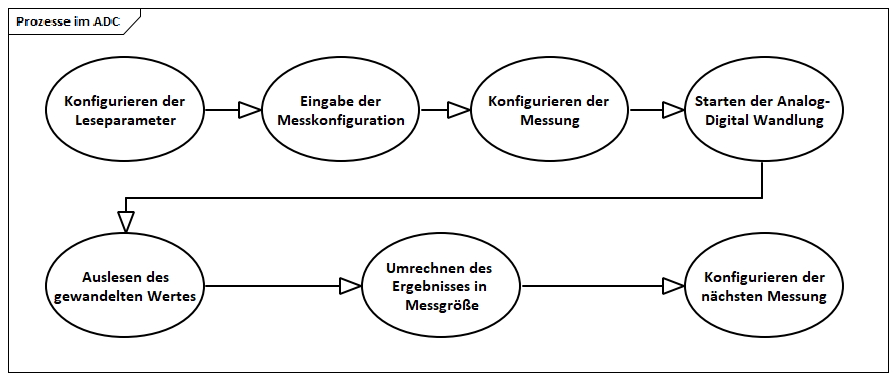
\includegraphics[width=1\textwidth]{Figures/Chapter_3/Prozesse im ADC.png}
    
    \captionof{figure}{Ablaufende Prozesse in einem AD- Wandler}
    \label{fig:adc-processes}
\end{figure}

Ziel des Frameworks ist allerdings, die Nutzung des Objektes einfach und intuitiv zu gestalten.
Demnach sollen nur die Prozesse dem Nutzer offenbart werden, die individuelle Konfiguration benötigen.
Technische Prozesse sollen weitesgehend verborgen bleiben.
Demnach sind nur folgende Aufgaben sichtbar:
\begin{itemize}
    \item Konfigurieren der wichtigsten Daten wie Datenrate
    \item Übergeben der Messkonfiguration
    \item Starten des AD- Wandlers
    \item Abrufen der gemessenen Daten.
\end{itemize}
Starten der einzelnen Messungen oder das Umrechnen, Verarbeiten und Testen von Daten geschieht autonom und wird bei Fehlern durch Diagnosewarnungen an andere interne Komponenten im Framework weitergegeben.
Der Nutzer des Frameworks muss sich keine Gedanken machen, wann Messungen gestartet werden und wann die Ergebnisse verfügbar sind.
Die Daten werden beim internen als auch beim externen \ac{adc} unterschiedlich im Hintergrund aktualisiert (Dazu mehr in den jeweiligen Kapiteln \autoref{subsubsec:external-adc-software} und \autoref{subsubsec:internal-adc-software}).

Die letztendliche Umrechung soll in Datenumrechnungsklassen stattfinden.
Diese werden in Form eines sogenannten Converters dem \ac{adc} übergeben.
Wird also zu einem späteren Moment vom Master das Signal gegeben, dass über den Eingang eine andere Größe gemessen wird, kann der Converter ausgetauscht und die Konfiguration geändert werden, ohne einen neuen ADC zu erstellen oder neue Firmware\footnote{Firmware beschreibt Software, die in elektronische Geräte fest implementiert ist. Sie ist im Gegensatz zu herkömmlicher Software mit der Hardware unzertrennlich verankert. Die Firmware wird auf einem Flash-Speicher, (z.B. einen EEPROM) gespeichert und ist vom Benutzer nicht ohne Weiteres auswechselbar. (Nach \textcite[][]{itservice.firmware}} zu schreiben.

Ein Problem bei der Ansteuerung zwei stark unterschiedlicher \ac{adc} ist die Messkonfiguration.
Der in dem Modul verbaute \textit{STM32G473} besitzt einen integrierten AD- Wandler, der intern die von STM bereitgestellte \textit{HAL- Bibliothek} benutzt.
Da dieser nur für das Messen der internen Spannungsversorgung und der CPU- Temperatur benutzt werden sollte, muss hier kein großer Wert auf die Konfiguration der Messungen gelegt werden.
Es reicht, lediglich den zu messenden Kanal und den \glqq Converter\grqq (Dazu mehr in \autoref{subsubsec:data-calculation-classes}) für die Umrechnung der gemessenen Spannung in eine reale Messgröße anzugeben.

Der extern auf dem Modul verbaute \ac{adc} hingegen ist für weit vielseitigere Anwendungsbereiche ausgelegt.
Auch muss er weitaus genauere Ergebnisse liefern, da er die Hauptaufgabe des Produktes übernimmt: Das Messen der an den Ports angelegten Spannungen.
Dafür sind demnach auch mehr Parameter für die Messkonfiguration notwendig:\newline
Das wären zum einen zwei an dem \ac{adc} verbaute Eingänge, über die die Spannung gemessen werden soll.
Die über diese beiden Bezugspunkte abfallende Spannung wird anschließend in die Messgröße umgerechnet.\newline
Zusätlich kann an dem Bauteil mehrere Referenzspannungen angelegt werden.
Somit kann eine von mehreren Referenzsspannungen ausgewählt werden.
Auch muss die Konvertierungszeit, im Datenblatt von Texas Instruments auch als Datentrate beschrieben, für verschiedene Messarten eingestellt werden. 
In \autoref{subsubsec:external-adc-software} wird genauer auf die zu beachtenden Messarten eingegangen.
Zuletzt muss auch das sogenante \textit{Gain}, der Verstärkungsfaktor des im ADS124S08 verbaute Operationsverstärkers eingestellt werden. Dieser ist notwendig, da das Produkt im Betrieb in der Regel sehr kleine Spannungen messen muss.

Da der externe \ac{adc} allerdings zusätzlich zu den oben genannten Eigenschaften auch die Konfigurationsparameter des internen \ac{adc} benötigt, kann man diese Konfigurationsstruktur weiterverwenden.
Da im \ac{adc} Interface ein gemeinsamer Datentyp als Parameter für die Konfigurationsmethode benötigt wird, kann man die gemeinsame Konfigurationsstruktur als eine Art \textit{Interface} nutzen.
Somit kann die Struktur des externen \ac{adc}, aber auch gegebenenfalls später folgende Strukturen, unter diesem Interface als einheitlicher Datentyp zusammengefasst werden. (Siehe in \autoref{lst:adc-conf-structs} \autoref{subsec:conf-structs-adc})

Beachtet man alle oben genannten Kriterien, dürfte das Interface letztendlich wie in \autoref{fig:adc-interface} aussehen.
Es beinhaltet einen Timer, da der ADC gemäß des \textit{Time Pattern} agieren soll.
Das heißt, dass nicht eine Messung gestartet wird und anschließend auf ein Ergebnis gewartet, sondern im Hintergrund aktuelle Daten zur Verfügung stehen.
Diese können dann mit der Methode \textit{getData} angefordert werden.
Eine genaue Erläuterung dieses Pattern ist beim externen \ac{adc} zu finden.

\begin{figure}[!htb]
    \begin{center}
        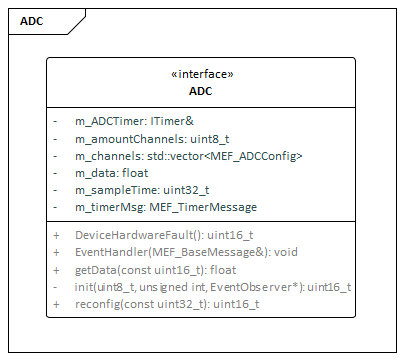
\includegraphics[width=0.7\textwidth]{Figures/Chapter_3/ADC.png}
        
        \captionof{figure}{Klassenstruktur des ADC Interfaces}
        \label{fig:adc-interface}
    \end {center}
\end{figure}

Das Attribut \textit{amoutChannels} dient nur zum Speichern der Länge des Messvektors, damit soll etwas Performanz gespart werden, da diese an vielen Stellen der Klasse benötigt wird.
Im \textit{data} Attribut wird das aktuelle Messergebnis zwischengespeichert.
Das Attribut \textit{sampleTime} beinhaltet die konfigurierte Wandlungszeit und in \textit{MEF\_TimerMessage} wird die Nachricht für das Aufsetzen eines neuen Timers abgespeichert.
Da der Timer nicht Umfang dieser Arbeit ist, wird er in \autoref{subsubsec:external-adc-software} bei der Implentierung des Timepatterns nur kurz umschnitten.

Die Methode \textit{DeviceHardwareFault} ermittelt die korrekte Arbeitsweise des \ac{adc}s und wird in der gleichnamigen Diagnose ausgewertet (Siehe \autoref{sec:diagnosen}- Diagnosen).
Der Eventhandler wird wegen des eventgesteuerten Timers benötigt, um nach Ablauf dessen und Auswerten der Nachricht das Messergebnis korrekt auszulesen und umzurechnen.
Deutlich wird das in \autoref{subsubsec:external-adc-software} bei Erläuterung der Implementierung des Time Patterns.
Die Methoden \textit{init} und \textit{reconfig} dienen zur initialisierung und gegebenenfalls umkonfigurierung der \ac{adc}- Parameter.


\subsubsection{Der externe AD- Wandler}
\label{subsubsec:external-adc-software}
Der externe \ac{adc} kapselt sich in drei Klassen, von denen eine abstrakt ist und zwei konkret.
Eine der beiden konkreten Klassen fungiert dabei nur als Treiber des externen AD- Wandlers.
Einschränkungen des im Folgenden dargestellten Treiber- Konzepts wird in \autoref{subsubsec:analysis}-Vergleich und Analyse einer zweiten Lösung aufgezeigt und diskutiert.

Um ein Objekt für den externen ADC zu erzeugen, muss man einen Sensorobjekt erstellen.
Dieser Sensor verbildlicht das Messen der Größe.
Somit muss der Nutzer nicht wissen, wie analoge Größen gemessen werden, sondern lediglich dass der Sensor mit gewissen Messparametern ein Ergebnis produziert, dass weiterverwendet werden kann.
Ein Sensor misst eine Größe- also wird auch ein Sensor erzeugt.

Intern startet der Sensor (In diesem Beispiel ist es der \ac{rtd}- Sensor zum Messen einer Temperatur) den \ac{adc} und konfiguriert diesen.
Die Messwertbereitstellung geschieht über das Timepattern, welches anhand des Programmcodes in dem Kapitel RTDSensor- Klasse genauer beschrieben wird.

Im Folgenden werden der Aufbau und die Funktion der einzelnen Klassen genauer beschrieben:

\minisec{ExternalADC- Klasse}
Der externe \ac{adc} dient zur Kapselung der Funktionalität, die alle externen \ac{adc}s zusammen haben: Die Kommunikation zwischen Wandler und der Firmware, die auf der CPU abläuft und technische Konstanten, die für das Setzen und auslesen einzelner Bits in den Registern \ac{adc}s benötigt werden (Jedes Register beinhaltet 8 Bits).
EIn Überblick dieser Funktionen ist in \autoref{fig:external-adc} zu sehen.

\begin{figure}[!htb]
    \begin{center}
        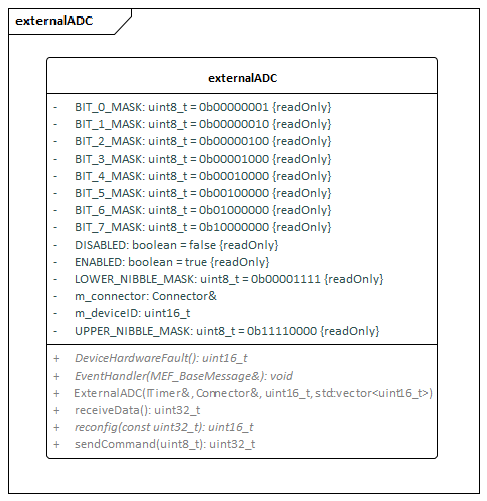
\includegraphics[width=0.7\textwidth]{Figures/Chapter_3/externer_adc.png}
        
        \captionof{figure}{Klassenstruktur des abstrakten Klasse des externen ADC}
        \label{fig:external-adc}
    \end {center}
\end{figure}

Im Konstruktor wird der Klasse ein Objekt des Typs \glqq Connector\grqq übergeben.
Der Connector ist dabei kein spezifisches Objekt, sondern ein Interface für beliebige Kommunikationsprotokolle.
In diesem Framework stehen dazu der \textit{\ac{spi}- Bus} und der IOLink- Stack für die Kommunikation zur Verfügung.
Der IOLink- Stack wird allerdings nur zur Kommunikation des Moduls mit dem Master genutzt.
Intern können keine Bauteile mit dem IOLink Stack angesprochen werden.
Auf der Hardware wird das \ac{spi}- Protokoll zur Bauteiladressierung genutzt.
Dementsprechend wird in der Hauptapplikation des Projekts dem \ac{adc} ein Connector des Typs SPI übergeben.\newline
Zusätzlich zu diesem Kommunikationsmodul wird eine sogenannte \glqq Device ID\grqq benötigt.
Das ist eine einmalig vergebene Zahl, mit der ein Bauteil direkt identifiziert werden kann.

Der Konnektor wird in den Methoden \textit{sendCommand} und \textit{receiveData} benötigt.
Diese sollen die Kommunikation eines externen AD- Wandlers mit der \ac{cpu} kapseln.
Dabei wird in den Methoden jeweils eine vom Framework definierte Nachricht (\textit{MEF\_SPIMessage}) gebaut.
In diese wird die Device ID hinzugefügt.
Zusätzlich wird bei der Methode sendCommand der Befehl mit seiner Speichergröße (Command- Parameter) oder bei der Methode receiveData Speicherplatz für die gelesenen Daten zugewiesen.
Bei dem Empfangen der Daten muss zuätzlich die Antwort des AD- Wandlers umgeformt werden.
Dieser sendet den digitalen Wert in einem Byte- Array.
Mit dem Algorithmus aus \autoref{lst:array-to-int-code} wird das Byte- Array in eine \textit{uint32\_t} Variable konvertiert.

Weiterhin instanziiert die Klasse ein Timerobjekt des Typs ITimer.
Dieses wird für das bereits erwähnte Time- Pattern in der Klase RTD- Sensor benötigt.
Da in der Regel allerdings alle externen AD- Wandler dieses Pattern nutzen werden, kann das Timerobjekt bereits hier gespeichert werden.
Implementiert werden kann das Pattern allerdings noch nicht, da dazu ebenfalls Zugriff auf die spezifischen Messkonfigurationen benötigt wird.
Da nicht jeder externe \ac{adc} zwingend das gleiche Konfigurationsobjekt nutzen wird, steht dieses nur in der Klasse RTDSensor zur Verfügung.

Auch ITimer ist ein Interface.
Timer sind in der Regel auf der \ac{cpu} verbaut.
Daher können diese beim Wechsel auf eine neue CPU anders implementiert werden müssen.
Im aktuellen Projekt stehen die Timer des Prozessors STM32G473 sowie Softwaretimer zur Verfügung.
Softwaretimer sind dabei lediglich schnelle ein schneller Timer, auf den sich mehere Objekte einschreiben können.
Diese werden nur alle n Takte benachricht (Wenn ein Timer zum Beispiel jede Sekunde abläuft, aber ein Objekt nur alle fünf Sekunden benachrichtigt werden muss, wird dieses nur jedes fünfte Mal benachrichtigt).

\minisec{ADS124S08- Klasse}
Die ADS124S08- Klasse ist zwischen dem externen \ac{adc} und dem RTDSensor platziert und stellt sämtliche Hardwarefunktionen zur Verfügung, die für die Benutzung des AD- Wandlers benötigt werden.
Zusätzlich enthält dieses Klasse die aktuelle Konfiguration des Wandlers.
Die Komplette Klassenstruktur ist in \autoref{fig:ads124s08-classdiagramm} zu sehen.\newline
Im Folgenden werden nur die für die Messung eines Wertes notwendigsten Werte eingegangen.
Andere Methoden wurden im Nachgang von einem Hardwareentwickler des Unternehmens hinzugefügt.

Im Allgemeinen sind die Methoden zum Setzen und Lesen von Konfigurationsparametern sehr ähnlich:
Zuerst wird eine Registeradresse benötigt. Diese bestimmt das Register, in dem der Konfigurationswert gesetzt wird.

Da meist nie das ganze Register neu gesetzt wird, sondern nur einzelne Bits darin geändert werden, muss zuerst der aktuelle Wert des Registers ausgelesen werden.
Der gelesene Wert wird mit einer Bitmaske bitweise verundet, um einzelne Bits zu extrahiern.
Diese können danach mit einem bitweise Oder gesetzt werden.\newline
Ist somit der neue Registerwert gebaut, kann dieser erneut in das Register geschrieben werden.

\begin{figure}[!htb]
    \begin{center}
        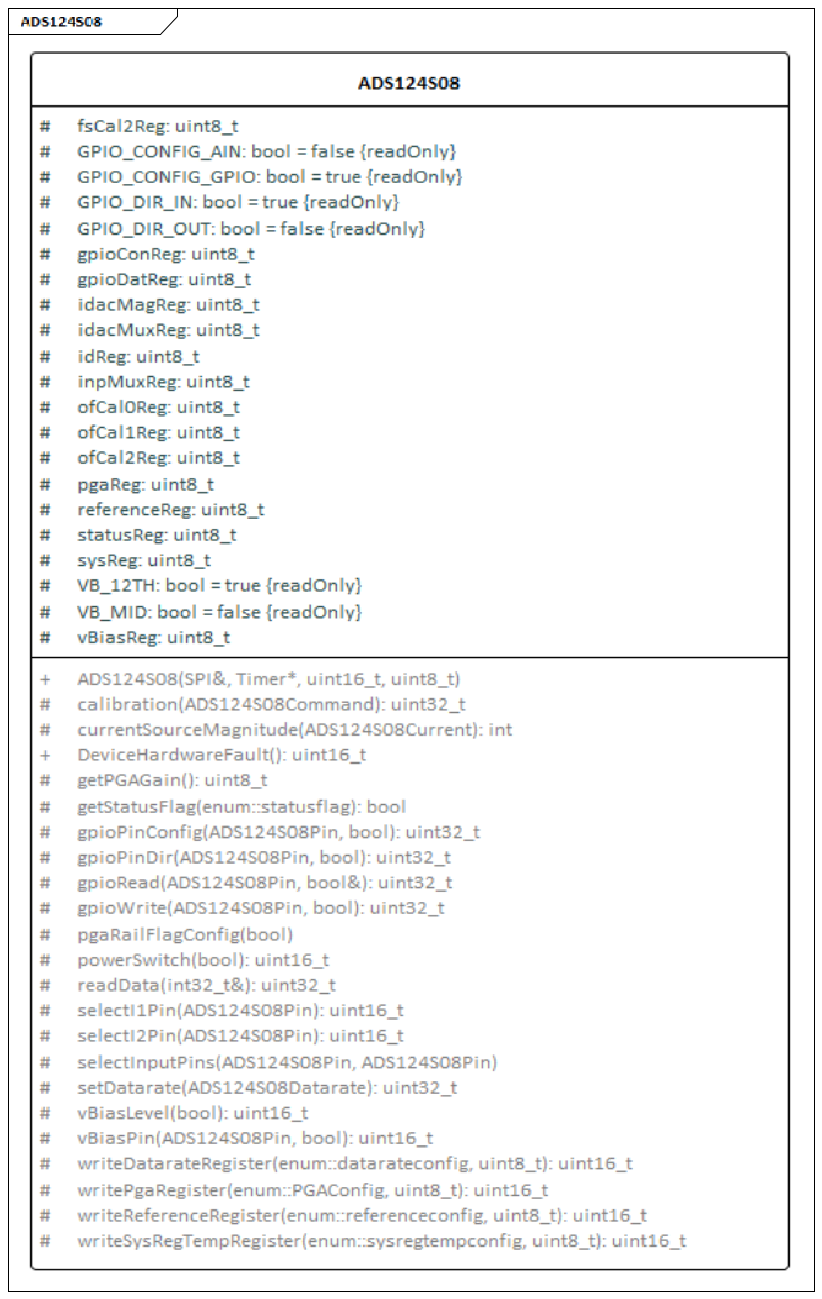
\includegraphics[width=0.7\textwidth]{Figures/Chapter_3/ADS124S08.png}
        
        \captionof{figure}{Klassenstruktur des ADC- Treibers}
        \label{fig:ads124s08-classdiagramm}
    \end {center}
\end{figure}

Um das ganze nochmals zu verdeutlichen, wird der Code am Beispiel der Methode \textit{pgaGain(ADS124S08PGAGain gain)} durchgesprochen.
Der Code für diese Methode ist in \autoref{lst:pga-conf} zu sehen.

Bei dem Parameter gain handelt es sich dabei um ein im Framework deklariertes Enum.
Der intern verbaute Operationsverstärker ist zwar konfiguerierbar, lässt allerdings nur die Werte 1, 2, 4, 8, 16, 32, 64 und 128 zu.
Deshalb wurde für den Nutzer die Eingabe eines Verstärkungsfaktors durch dieses Enum auf ebendiese Werte beschränkt.

\begin{lstlisting}[caption={Neukonfigurieren des intern verbauten Operationsverstärkers}, label=lst:pga-conf]
uint32_t ADS124S08::pgaGain(ADS124S08PGAGain gain) {
	uint8_t pgaRegTemp = m_pgaReg;
	pgaRegTemp &= ~(BIT_2_MASK | BIT_1_MASK | BIT_0_MASK);
	pgaRegTemp |= (uint8_t)gain;

	uint32_t error = writeReg((uint8_t)ADS124S08RegAddr::PGA_ADDR, pgaRegTemp);

	if(!error) {
		m_pgaReg = pgaRegTemp;
	}

	return error;
}
\end{lstlisting}

Da Treiber nicht nur die Hardwarefunktionen für die Bedienung des \ac{adc} breitstellt, sondern auch diesen auf Hardwareebene repräsentiert, müssen die jeweiligen Registerwerte erst ausgelesen werden.
Stattdessen wird der Inhalt der Register in verschiedenen Attributen abgespeichert.
Damit kann die Zeit, die zum auslesend er Daten über \ac{spi} benötigt wird, gespart wird.

Die oben genannten Verstärkundsfaktoren sind von null aufsteigend numerisch kodiert.
Die Kodierung für den Verstärkungsfaktor 64 ist beispielsweise 110.
Da es acht verschiedene gibt, werden drei Bit für diese Kodierung benötigt.
Diese drei Bit befinden sich in den untersten drei des Registers.
Um diese zu Maskieren, werden in Codezeile drei die Bitmasken der Bits eins, zwei und drei bitweise verodert: Das Ergebnis ist \textbf{00000111}.
Wird diese Maske mithilfe der Tilde bitweise invertiert, ergibt sich \textbf{11111000}.
Eine bitweise Verundung mit dem Registerwert setzt somit alle Stellen, die den Verstärkungsfaktor definieren, auf Null.
Das Ergebnis dieser Operation ist \textbf{xxxxx000}.

Wird nun der ganzzahlige Wert des mitgegebenen Verstärkungsparameter (der durch einfaches Casten aus dem Enum erhalten werden kann) mit dem neuen bitweise Verundet, erhält man den neuen Wert des Registers.
Bei einem Verstärkungsfaktor von 64 wäre das \textbf{xxxxx110}.

Dieser Wert kann nun in das Register geschrieben werden (siehe Codezeile 6).
Ist der resultierende Fehlercode \textit{MEF\_ERROR\_NO\_MALFUNCTION}, intern kodiert als 0x0000, wurde der Wert erfolgreich in das Register geschrieben.
Das Klassenattribut für dieses Register kann nun durch den neuen Wert ersetzt werden (Siehe Codezeile 9).

\minisec{RTDSensor- Klasse}
Die Hauptaufgabe der \ac{rtd}- Sensors ist das Managen der Messungen, die über den ADS124S08 durchgeführt werden.
Namensgebend für die Klasse ist der gewünschte Messvorgang: Das Messen der Temperatur über \ac{rtd}- Sensoren.
Eine Übersicht der Klasse ist in \autoref{fig:rtd-classdiagramm} zu finden.

\begin{figure}[!htb]
    \begin{center}
        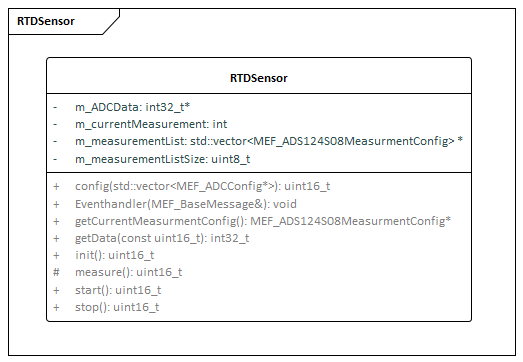
\includegraphics[width=0.7\textwidth]{Figures/Chapter_3/RTDSensor.png}
        
        \captionof{figure}{Klassenstruktur des RTD- Sensors}
        \label{fig:rtd-classdiagramm}
    \end {center}
\end{figure}

Die Klasse bietet die Möglichkeit, die Messungen zu starten oder zu stoppen.
Ist der Messvorgang erstmal gestartet, werden im Hintergrund die Daten nach erfolgreicher Umwandlung des Bauteils aktualisiert.
Wird in der Software also ein Wert gebraucht, kann dieser direkt aus der Klasse extrahiert werden.\newline
Zusätzlich kann der RTD- Sensor initialisiert werden, indem eine Testmessung stattfindet.
Wichtig jedoch sind die \textit{config}- Methoden.
Ihnen wird ein Vektor mit Messkonfigurationsstrukturen (wie in \autoref{subsec:hardware} bereits besprochen) übergeben.
Diese Methode ersetzt die alte Reihenfolge der Messungen mit der ihr Übergebenen.
Das ganze kann dynamisch zur Laufzeit geschehen.
So kann auf Nachrichten des IOLink Masters reagiert werden und Messungen entfernt, geändert oder hinzugefügt werden.

Kern der Klasse ist der Eventhandler. In ihm wird das Time Pattern implementiert.
Dadurch wird erreicht, dass nur Rechenzeit benötigt wird, um ein Messergebnis zu bearbeiten und eine neue Messung zu starten.
Ein Überblick über die Abläufe des Eventhandlers liefert \autoref{fig:rtd-ablauf}.

Der erste dort abgebildetete Schritt, das Initialisieren des AD- Wandlers, führt der Nutzer noch selbst durch.
Der folgende Teil wird läuft im Hintergrund ab.

Zuerst wird der Timer gestoppt.
Danach wird dieser mit einer neuen Zeit initialisiert.
Diese ergibt sich aus der eingestellten Wandlungszeit aus der Messkonfiguration (siehe \textcite[][42]{TexasInstruments.2016}).\newline
Anschließend wird dem Timer der Eventhandler selbst mitgegeben.
Das ist nur das erste mal nach dem Starten der Firmware notwendig.

Ist der Timer soweit konfiguriert, kann dem AD- Wandler der Befehl zum starten der neuen Wandlung gegeben werden.
Dazu wird eine weitere Methode aufgerufen: In ihr werden all die Attribute aus der aktuellen Messkonfiguration in die Register des \ac{adc}s geschrieben.\newline
Anschließend wird der STOP- Befehl gesendet, um den Wandler zu pausieren und folgend wieder mit dem START- Befehl zu aktivieren.
Nun wird die Wandlung mit der neuen Konfiguration durchgeführt.

Nach Aufruf dieser Methode bleibt im Eventhandler nur nach das Starten des oben konfiguerierten Timers.
Dieser sollte erst nach dem Starten der Messung aktiviert werden, da damit Sichergestellt ist, dass er nach Beenden der Wandlung ein Interrupt startet.

Danach beendet sich der Eventhandler im ersten Durchlauf und überlässt die Rechenzeit der \ac{cpu} anderen Teilen der Software.
Erst beim Ablaufend der Timer wird der Eventhandler erneut aufgerufen.

\begin{figure}[!htb]
    \begin{center}
        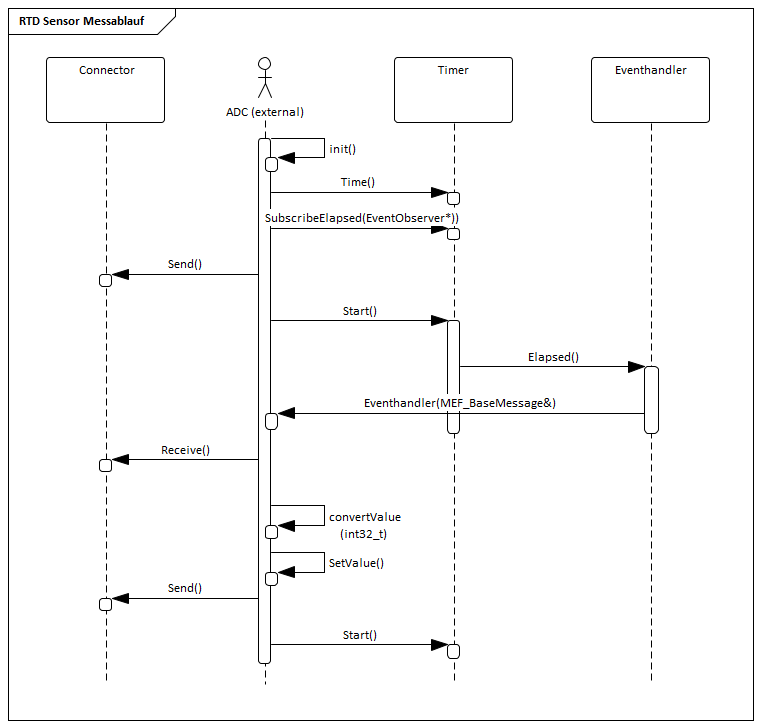
\includegraphics[width=1\textwidth]{Figures/Chapter_3/rtd-ablauf.png}
        
        \captionof{figure}{Ablaufdiagramm über das bereitstellen neuer Daten}
        \label{fig:rtd-ablauf}
    \end {center}
\end{figure}

Da nun bereits eine Messung stattgefunden hat, ist der erste Schritt nicht mehr das neu konfigurieren der des Timers.
An dieser Stelle wird das aktuell am \ac{adc} zwischengespeicherte Ergebnis abgerufen.
Das passiert mit der ReceiveMethode, bei der zusätzlich über \ac{spi} nicht nur der READ- Befehl gesendet wird, sondern auch ein Array mit dem benötigten Speicherplatz, um das Messergebnis zwischen zu speichern.
Um der hohen Auflösung des Bauteils gerecht zu werden, wird dazu ein Array aus drei vorzeichenlosen Acht- Bit- Integer- Werten benutzt.

Wie bereits erwähnt, wird dieser Wert direkt in ein 32- Bit Integer Wert gewandlet (siehe \autoref{lst:array-to-int-code} in \autoref{subsec:array-to-int-code}) und kann direkt weiterverarbeitet werden.
Das geschieht in den sogenannten Datenumrechnungsklassen in \autoref{subsubsec:data-calculation-classes}.
Der Eventhandler nutzt nochmals die Konfigurationsstruktur der vorherigen Messung. Die dortige Umrechnungsklasse beinhaltet eine \textit{convert(uint32\_t)} Methode, die den Messwert in eine reale Messgröße umrechnet.

Ist dieser Wert nun umgerechnet, kann dieser in dem Array an seiner jeweiligen Position abgespeichert werden.
Über die Methode getData kann dieser Wert nun abgerufen und außerhalb der Klasse weiterverwendet werden.

Nun werden die oben erläuterten Schritte erneut durchgeführt und somit die nächste Messung gestartet.

\subsubsection{Der interne AD- Wandler}
\label{subsubsec:internal-adc-software}

Der interne AD- Wandler ist direkt auf dem CPU verbaut.
Im Umfang des Porojektes dient er zur internen Versorgungsspannung- sowie Referenzspannungsüberwachung.
Das Messen der intern vorliegenden Referenzspannung dient dem genaueren Messen mit dem externen AD- Wandler: Wie so viele andere Größen unterliegt auch die Referenzspannung Schwankungen über der Zeit.
Um somit den aktuellen Referenzwert möglichst genau zu haben, wird für die Referenz anstelle der idealerweise volriegenden Spannung, die nur auf ein Zentel Milivolt genau spezifiziert ist, ein deutlich genauerer Wert verwendet, der die aktuelle Abweichung retuschiert.

Er kommunizert direkt mit der \ac{cpu}.
Daher kann er diese auch über einen direkten Speicherbus: Den \ac{dma}- Bus.
Dieser sichert eine höhere Ausführungsgeschwindigkeit laufender Programme.

Zum einen muss der Prozessor nicht erst Daten in die eigenen internen Register einlesen, um sie direkt wieder in den Arbeitsspeicher zu schreiben, sondern die Daten über eine spezielle Datenleitung zwischen der Hardware senden.
beispielsweise benötigt ein Speichertransfer über den Prozessor in der Regel ungefähr 40 Takte.
Über \ac{dma} kann das innerhalb von vier Takten geschehen. (nach \textcite[][]{ElektronikKompendium.DMA})

Zum anderen kann speziell im Anwendungsfall der Analog- Digital Umwandlung Zeit gespart werden.
Der interne AD- Wandler kann mit den verschiedenen auszuführenden Messungen programmiert werden und in den sogenannten \textit{Continious Mode} gesetzt werden.\newline
Das heißt, er führt die einzelnen Messungen der Reihe nach immer wieder erneut durch, bis die Stromversorgung versiegt.
Die Ergebnisse der Wandlung müssen auch nicht erst am Bauteil abgeholt werden, sondern stehen direkt im Arbeitsspeicher.
So muss sich die Software nur einmal initial um den Wandler kümmmern und anschließend nur noch wenn die Messungen geändert werden sollen.

STM liefert zu den hauseigenen \ac{mcu}s eine Softwarebibliothek um diese anzusteuern: Die HAL- Bibliothek.
Aktiviert man in dieser Bibliothek den internen AD- Wandler der \ac{mcu}, stellt die HAL- Bibliothek ein \textit{Handle}\footnote{ Referenzwert einer Ressource, das durch ein bestimmtes System verwaltet wird} zur Verfügung, über das der \ac{adc} konfiguriert und angesprochen werden kann.

Wird der Kanal gewechselt, muss dieser über das Handle umgeschrieben werden.
Dafür ist die private Methode \textit{configChannel} in \autoref{fig:internal-adc} zuständig.\newline
Dort wird ein neues \textit{ADC\_ChannelConfTypeDef}- struct erstellt, dass unter anderem ein Attribut für den Kanal oder auch die Konvertierungszeit hat.
Mit der von HAL zur Verfügung gestellte Funktion \textit{HAL\_ADC\_ConfigChannel(adc\_handle, \&sConfig\_struct)} kann die Konfiguration in das Handle geschrieben werden und somit einen neuen Kanal messen.

\begin{figure}[!htb]
    \begin{center}
        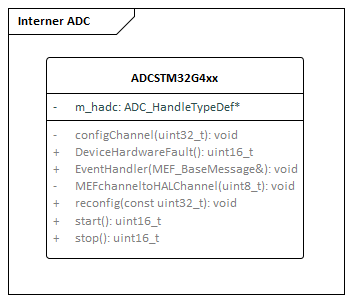
\includegraphics[width=0.65\textwidth]{Figures/Chapter_3/Interner ADC.png}
        
        \captionof{figure}{Klassendiagramm des internen \ac{adc}}
        \label{fig:internal-adc}
    \end {center}
\end{figure}

Dabei muss beim Messen mehrerer Kanäle allerdings nicht regelmäßig der Kanal geändert werden.
Beim Verwenden von \ac{dma} sollte im Anwendungsfall mehrerer Kanäle der sogenannte \textit{Multimode} akitiviert werden.
Mithilfe verschiedener Rängen kann in den Konfigurationen sichergestellt werden, dass die Kanäle nicht überschireben werden.
Ein Beispiel des Messens mehrerer Kanäle ist in \autoref{lst:multimode-adc} in \autoref{subsec:adc-multimode} dargestellt.

Da bei der Initialisierung der Treiber der HAL- Bibliothek das ADC- Handle mit einem \ac{dma} Handle verknüpft wird \footnote{Die Funktion lautet \_\_HAL\_LINKDMA(adcHandle, DMA\_Handle, hdma\_adc1)}, muss das \ac{dma}- handle nicht weiter zur Konfiguration an die \ac{adc}- Klasse weitergeleitet werden- alles relevante wird über das ADC- Handle konfiguriert unnd verknüpft.

Des weiteren beinhaltet die Klasse einen Methode \textit{MEFchanneltoHALChannel}, welche Frameworkinterne Definitionen der \ac{adc}- Kanäle auf die HAL- internen Definitionen abbildet.
Damit kann das Framework eigene Definitionen verwenden, die nicht so lang wie die der HAL- Bibliothek sind und anstatt den Namen der HAL- Bibliothek den des Frameworks enthalten.

Die weiteren Methoden der Klasse sind bereits aus obigen Erläuterungen bekannt und werden deswegen an dieser Stelle nicht mehr aufgeführt.


\subsubsection{Datenumrechnungsklassen}
\label{subsubsec:data-calculation-classes}
Da in diesem Framework Wiederverwendbarkeit an wichtigster Stelle steht, müssen einzelne Bearbeitungsschritte austauschbar gestaltet werden.
In diesem Zug wurde die Umrechnung modular für jede Messung konzipiert.
Das bedeutet, dass sie auf Konfigurationsebene für jede Messung angegeben werden muss.

Dabei hat es nicht gereicht, eine Umrechnung als Enum- Value anzugeben, der intern in der Klasse die Umrechnungsformel angibt.

Deswegen wurde diese Formeln in jeweils einer eigenen Klasse gekapselt.
Das bringt den Vorteil, dass sie nicht nur an anderen Stellen der Firmware wiederverwendbar zur Verfügung stehen und der Nutzer diese gegebenenfalls in eigenen Applikationen benutzen kann, sondern auch  dass im Notfall neue Umrechnungen geschrieben werden können, ohne Änderungen am \ac{adc} vornehmen zu müssen.\newline
Dies entspricht ganz dem Prinzip der Softwareentwicklung \textbf{Seperation of Concerns}: Das Umrechnen eines Wertes hat nichts mit dem Umwandeln eines analogen Wertes in einen digitalen Wert zu tun- es ist lediglich im Use Case der Anwendung notwendig, den Wert aufzubereiten.

Der Grundaufbau dieser Umrechnungsbausteine ist ein Konstruktor, über den alle zur Umrechnung wichtigen Konstanten übergeben werden und die Methode zum umrechnen des Messertes (siehe \autoref{fig:data-calc-class-diagramm}).

\begin{figure}[!htb]
    \begin{center}
        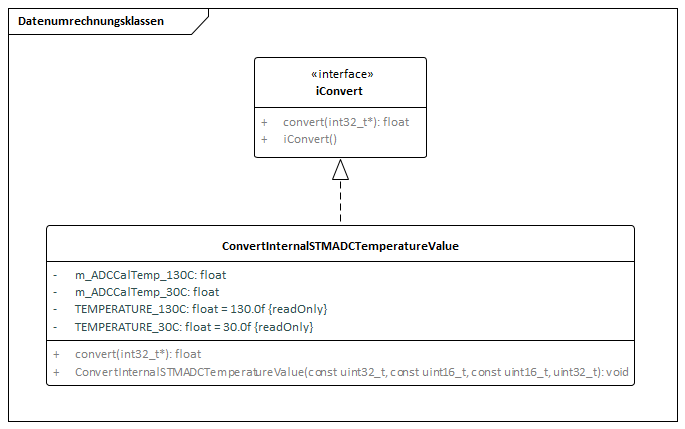
\includegraphics[width=1\textwidth]{Figures/Chapter_3/Datenumrechnungsklassen.png}
        
        \captionof{figure}{Beispielhafte Struktur einer Umrechnungsklasse mit dem Interface}
        \label{fig:data-calc-class-diagramm}
    \end {center}
\end{figure}

Konstanten sollten sich innerhalb der gleichen Messkonfiguration nicht ändern.
Dementsprechend bietet es sich an, diese über den Konstruktor an das Objekt zu übergeben.
Desweiteren hat es den Vorteil, dass der Konstruktor als einzige \glqq Methode \grqq nicht vom Interface erbt und somit auch nicht die gleiche Parameterstruktur im Funktionskopf beinhalten muss.
Somit kann jeder Konvertierungsklasse ein individueller Satz an Parametern übergeben werden.\newline
In \autoref{fig:data-calc-class-diagramm} wird beispielsweise die Referenzspannung des internen Ad- Wandlers als auch die bei der Produktion getesteten Kalibrierungswerte übergeben.
Im Konstruktor werden daraufhin die beiden Konstanten m\_ADCCalTemp\_30 und m\_ADCCalTemp\_130 aus diesen Werten berechnet.
Mit diesen beiden Konstanten ergibt sich darauf die Formel aus \autoref{lst:intern-temp-value}.

\begin{lstlisting}[caption={Formel zur Berechnung der Betriebstemperatur}, label=lst:intern-temp-value]
(static_cast<float>(*data) - m_ADCCalTemp_30C)/(m_ADCCalTemp_130C - m_ADCCalTemp_130C) * (TEMPERATURE_130C - TEMPERATURE_30C) + TEMPERATURE_30C;
\end{lstlisting}

Der Umrechnungsmethode wird ein Pointer des Typs uint32\_t übergeben.
Damit stellt das Interface sicher, dass Klassen, die zwei Werte zur Umrechnung benötigen, diese auch im Funktionskopf in Form eines Array annehmen können.

In \autoref{fig:data-calc-class-diagramm} wird das nicht benötigt. 
Allerdings kann es im Fall der Drei- Leiter Messung (siehe \autoref{subsubsec:external-adc}) ist dies wichtig.

Eine Anforderung an das Projekt war, zur Laufzeit dynamisch auf Änderungen zu reagieren.
Auch das ist gewährleistet.
Ändert sich zum Beispiel am externen AD- Wandler ein angeschlossener Sensor von beispielsweise einem PT100 (Platindraht mit Basiswiderstand von 100 Ohm) zu einem NI200 (Nickeldraht mit Basiswiderstand von 200 Ohm), so kann darauf reagiert werden, indem in der jeweiligen Messkonfigurationsstruktur zur Laufzeit das Datenumrechnungsobjekt mit dem des neuen Sensors ausgetauscht wird.

Weitere Umrechnungsklassen, die für die Anforderung des Projektes geschrieben wurden, umfassen das Konvertieren des Bitwertes in die Betriebsspannung des Moduls oder in die intern vorliegende Referenzspannung.
Beide Umrechnungen funktionieren weitesgehend analog zu der vorgestellten Formel.

Weiter sind aber auch Umrechnungen für den externen AD- Wandler benötigt.
Dieser muss den gemessenen Wert in einen Widerstand umrechnen.
Der aktuelle Widerstand ist abhängig von der Temperatur und repräsentiert somit ebendiese.
Dieser Widerstand muss daraufhin auf den des Basissensors (PT100) herunter gerechnet werden und kann daraufhin erst in eine Temperatur gefomrt werden.\newline
Da im Lastenheft des Produktes mehrere Sensoren aufgelistet sind, mit denen das Modul funktionieren soll, ist diese Klasse stark von dem ausgewählten Sensor abhängig.
Ebenso ist die Klasse aber auch abhängig vom eingestellten Verstärkungsfaktor des integrierten Operationsverstärkers.\newline
Weitere Parameter, die der Klasse im Konstruktor übergeben werden müssen ist die Art der Verdrahtung des Sensors.

In der Convert- Methode wird daraufhin folgend vom ersten gemessenen Widerstand (dem Gesamtwiderstand der Messchaltung) zweimal der zweite Widerstand (Leitungswiderstand, zweimal für Leitung vor- und nach dem Sensor) abgezogen. 
Daraus wird der Widerstand berechnet und abhängig vom Sensortyp die Temperatur berechnet.
Die Formeln dazu sind den Datenblättern entnommen.
Der Programmcode für diese Umrechnung ist zu umfassend, um in dieser Ausarbeitung als Listing aufgeführt zu werden.


\subsubsection{Vergleich und Analyse einer weiteren Lösung}
\label{subsubsec:analysis}
Während der Theoriephase des vierten Semesters wurde die Programmstruktur des AD- Wandlers von einem weiteren Softwareentwickler des Unternehmens während der Applikationsentwicklung für ein zweites Produkt überarbeitet.
Im Zuge dessen wurde eine Analyse beider Problemlösungen durchgeführt, um aus beiden das Beste für das Projekt zu extrahieren und eine Lösung beziehungsweise eine Mischform beider Entwürfe für das Framework zu finden oder Schwächen beider Lösungen aufzudecken.
